%%This is a very basic article template.
%%There is just one section and two subsections.
\documentclass[a4paper]{article}

\usepackage{geometry}         % Définir les marges
\usepackage{graphicx}
\usepackage{subcaption}

\title{NA62 RunControl}
\author{Nicolas Lurkin}

\newcommand{\note}[1]{\footnote{TODO: {#1}}}

\begin{document}

\maketitle

\section{Finite State Machine}
THe NA62 RunControl is based on a three levels tree-like hierarchy of Finite State Machine (FSM). 

Each constituting element of the DAQ (device) is internally modeled as an FSM. Each state of the
FSM is defined by the evaluation of logical expressions depending on a set of parameters that are
provided by the device. The figure \ref{fig:FSM_Device} shows the FSM diagram followed by most of
the devices.

The device nodes are forming the leaves of the tree that are grouping the devices into logical
entities representing subsytems of the experiment. These nodes are also modeled as FSM, summarizing
the states of the devices belonging to this group according to a set of rules.

Finally the root of the tree is an FSM node that represents the global state of the Data Acquisition
by further summarizing the states of all the logical nodes. The figure \ref{fig:FSM_Main} shows the
FSM diagram for this root node which is derived from the device FSM. The possible states are
described below:

\begin{figure}[hn]
	\centering
	\begin{subfigure}{0.4\textwidth}
		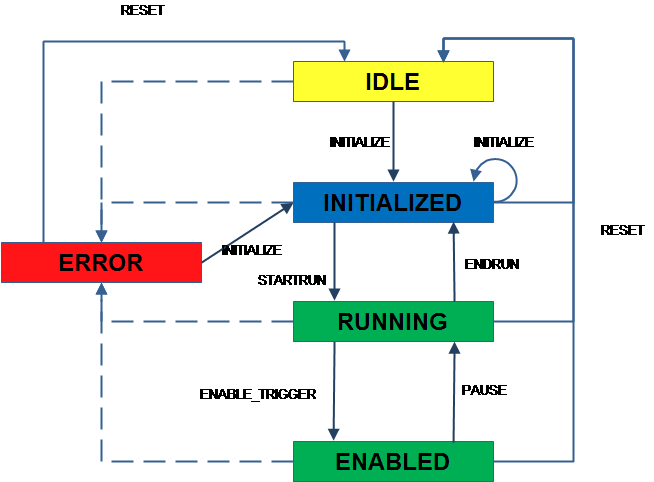
\includegraphics[width=\textwidth]{Doc/NA62FSM2.png}
		\caption{Generic FSM diagram for the devices.}
		\label{fig:FSM_Device}
	\end{subfigure}
	\begin{subfigure}{0.4\textwidth}
		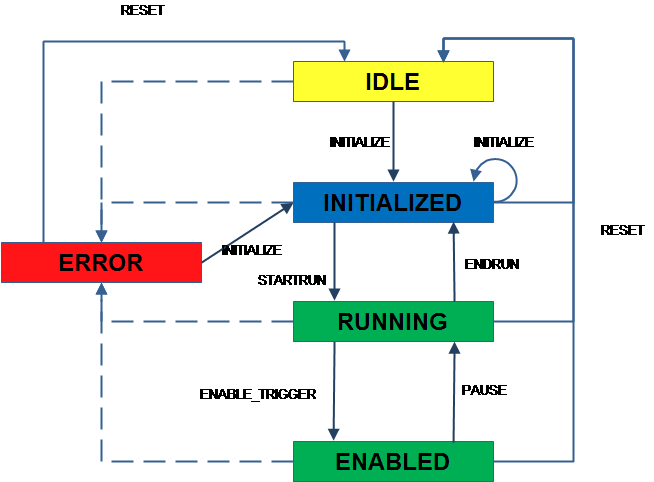
\includegraphics[width=\textwidth]{Doc/NA62FSM2.png}
		\caption{FSM diagram of the root node representing the global state of the NA62 DAQ}
		\label{fig:FSM_Main}
	\end{subfigure}
\end{figure}

\begin{itemize}
	\item \textbf{IDLE}: This is the initial state after starting or resetting the FSM and the devices.
	\item \textbf{INITIALIZED}: When all the devices have been configured and the DAQ is ready to take
	data.
	\item \textbf{RUNNING}: All the devices are completely running and waiting for triggers. The only
	exception being the trigger processor, in a paused state, waiting for further command to generate
	the triggers.
	\item \textbf{ENABLED}: The trigger processor is out of the paused state and running.
	\item \textbf{ERROR}: This state can be reached from any other state whenever a problem occurs on
	any device.
\end{itemize}

Each state allows a list of abstract commands that are propagated downward in the hierarchy to
the device nodes where it is transmitted through the network. The list of commands is described
hereafter:

\begin{itemize}
	\item \textbf{INITIALIZE}: Request to initialize all the devices with a specific configuration.
	\item \textbf{STARTRUN}: Request to all the devices to start the run and move in a ready state
	where they are able to take data.
	\item \textbf{ENABLE\_TRIGGER}: Request to the trigger processor to start generating triggers.
	\item \textbf{PAUSE}: Request to the trigger processor to stop generating triggers.
	\item \textbf{ENDRUN}: Request to all devices to stop taking data and end the current run. 
	\item \textbf{RECOVER}:  
	\item \textbf{RESET}: Immediately move to an idle/initialized state, stopping the current run if
	it was ongoing.
\end{itemize}

\section{Interface}
The link between the device nodes modelling a specific device and the hardware itself is
established by DIM\footnote{Distributed Information Management System}\note{link to dim} that will
take care of transmitting the commands from the RunControl to the device and the state parameters from the
device to the RunControl, along with any other relevant information that should be known by the
RunControl or made availabe to the shifters.

As the RunControl is not aware of the internal operation of any device the commands are very generic
and the device is expected to understand it and execute the appropriate sequence of actions
specific to itself. After the execution of the associated action the devices should answer back to
the RunControl, notifying the success or failure of the action.
 

The minimum set of commands to be understood and implemented is the following:
\begin{itemize}
  \item 
\end{itemize}

The state changes are triggered


(currently PC farm node, L0TP)

\section{Configuration}
The configuration mechanism of the RunControl will take advantage of the existing recipe mechanism
of the JCOP\note{Link to JCOP} framework: a database contains an ensemble of fields and a list of
recipes (configuration modes). Specific values of the field are associated to each recipe. At
configuration time a prompt will ask the user to select a recipe to load.

Again, in order to hide the internals of the devices from the RunControl, the actual configuration
parameters/values are contained in a configuration file. The content of the files will be written in
the JCOP database and associated to recipes. When loading a recipe, the associated files content
will be transmitted integrally to the device who will again be responsible to decode it and apply
the values.

A tool will be available to dump configuration files into the database and an ``on-line'' editor will
also be provided to modify/write files directly in the database. The entries in the database can be
independant files or different versions of a same file and will be identified by a name and will
be associated one or several tags relating it to recipes.

The configuration files can be incremental: for each recipe, a list of files can be sent to the
device. The first one would contain ``default'' values, values that are valid for different type of
runs, parameters that rarely change. The following files would contain parameters that have a higher changing rate.
The files will be send to the device sequentially and the value applied for a specific parameter
should always be the one specified in the last file (values in the latest file are overwriting the
values in the earliest ones). The default file could also be used when no file is specified for the
given recipe or when resetting the device.

The file transfer mechanism will work as described hereafter. After sending a command requiring a
configuration file, the RunControl will send the content of the first configuration file as a
string on a dedicated command slot. The RunControl will then wait until the device notifies it that
the file has been entirely processed and is waiting for further instructions. The RunControl will
repeat the same procedure for the next configuration files until the last one has been processed.

Once all the configuration has been applied the RunControl will ask the device to report back the
current configuration. The device will generate a file containing all the current parameters values,
possibly in the same format as the configuration file, that it will transmit to the RunControl. This
file will be stored in the offline database. Two possibilities are given to the subsystem:
\begin{itemize}
  \item When applying the configuration files, keeping track of the real value of each parameters
  (the one that has been applied) and report this list of values, trusting that everything went well
  and that these values were effectively loaded in the hardware.
  \item Request the hardware for the actual value of each parameter and report this list of true
  values.
\end{itemize}

When the complete procedure is finished the device should update it's state parameters and report an
INITIALIZED state in the RunControl. 

\section{Logging}
The RunControl will be connected to three different databases: the configuration database containing
the recipes and the configuration files, the online database storing number of information related
to the run and the instantaneous state of the data taking, PC farm, \ldots. And finally the offline
database that will contain the subset of the online values that are relevant to future analysis and
the configuration for each run.


\end{document}
